%Purpose:
%This is a beamer poster template. The original template (which I modified) came from Shawn Lankton (http://www.shawnlankton.com/tag/beamer/).
%
%Modified version by:
%Larz White, University of Idaho, Department of Physics: Nuclear Theory Group
%
\documentclass[serif]{beamer}
%============================packages and commands I use: remove/add them as necessary=============
\usepackage{graphicx,xfrac,mathtools,amssymb,braket,multirow,subfigure,float}
\newcommand{\bvec}[1]{\boldsymbol{#1}}%bold vectors
\newcommand{\rb}[1]{\left(#1\right)}%auto size round brackets
\newcommand{\sqb}[1]{\left[#1\right]}%auto size square brackets
\newcommand{\abs}[1]{\left|#1\right|}%absolute value
\newcommand{\avg}[1]{\left\langle#1\right\rangle}%average
\newcommand{\dd}{\,\mathrm{d}}%differential
%================Poster Layout: Make necessary changes========================================================
%orientation=landscape or portrait
%width(height)=set poster dimensions. Units are in cm. Thus, to get a 4ft x 3ft poster set width=120,height=90
%scale=font size in body of each block
\usepackage[orientation=landscape,size=custom,width=97,height=60,scale=0.57]{beamerposter}
%
%define rgb colors you want to use for poster theme
\definecolor{darkross}{rgb}{0.016,0.404,0.667}
\definecolor{middleross}{rgb}{0.020,0.522,0.859}
\definecolor{lightross}{rgb}{0.094,0.624,0.980}
\definecolor{darkblue}{rgb}{0.016,0.078,0.667}
\definecolor{middleblue}{rgb}{0.020,0.102,0.856}
\definecolor{lightblue}{rgb}{0.094,0.180,0.980}
\definecolor{darkpurple}{rgb}{0.604,0.016,0.667}
\definecolor{middlepurple}{rgb}{0.776,0.020,0.895}
\definecolor{lightpurple}{rgb}{0.894,0.094,0.980}
\definecolor{darkbrown}{rgb}{0.961,0.514,0.071}
\definecolor{middlebrown}{rgb}{0.725,0.557,0.271}
\definecolor{lightbrown}{rgb}{0.933,0.890,0.773}
\definecolor{darkolive}{rgb}{0.667,0.604,0.016}
\definecolor{middleolive}{rgb}{0.859,0.776,0.020}
\definecolor{lightolive}{rgb}{0.980,0.894,0.094}
\definecolor{darkgreen}{rgb}{0.078,0.667,0.016}
\definecolor{middlegreen}{rgb}{102,0.859,0.020}
\definecolor{lightgreen}{rgb}{180,0.980,0.094}
%
%setup blocks
	\setbeamercolor*{block title}{fg=black,bg=lightross}%block title font color
	\setbeamerfont{block title}{size=\large}%size of block title
	\setbeamercolor*{block body}{fg=black,bg=white}%font color in body of block. fg=text color, bg=block background
	\setbeamertemplate{block begin}{
	\begin{beamercolorbox}[rounded=true,shadow=true]{block title}
    \usebeamerfont*{block title}{\Large \insertblocktitle}%block title font size
    \end{beamercolorbox}
    \begin{beamercolorbox}[rounded=true,shadow=true]{block body}
    }
%
%setup headline
    \setbeamercolor{headline}{bg=white}%headline background color
    \setbeamercolor{title in headline}{fg=darkross}%title font color
    \setbeamercolor{author in headline}{fg=darkross}%author font color
    \setbeamercolor{institute in headline}{fg=darkross}%institute font color
    \setbeamertemplate{headline}{
    \begin{beamercolorbox}{headline}
    \begin{columns}[t]
    \begin{column}{.32\paperwidth}
    \end{column}
    \begin{column}{0.32\paperwidth}
    \vskip4ex
    \usebeamercolor{title in headline}{\centering \color{fg}\textbf{\Huge{\inserttitle}}\\[1ex]}
    \usebeamercolor{author in headline}{\centering \color{fg}\LARGE{\insertauthor}\\[1ex]}
    \usebeamercolor{institute in headline}{\centering \color{fg}\large{\insertinstitute}\\[1ex]}
    \end{column}
    \begin{column}{0.32\paperwidth}
    \begin{flushright}
    
\includegraphics[width=6.5cm,height=3cm]{logo}
    \end{flushright}
    \end{column}
    \end{columns}
    \end{beamercolorbox}
    }
%
%setup footline
    \newcommand{\footright}{\textit{*Email: whit2657@vandals.uidaho.edu}}%email in footline
    \newcommand{\footleft}{\textit{Presented at the 2012 UI student research exposition}}%note in footline
    \setbeamerfont{footline}{size=\large}%footline font size
    \setbeamercolor{footline more}{bg=white}%footline background color
    \setbeamercolor{email in footline}{fg=black}%footer1 font color
    \setbeamercolor{note in footline}{fg=black}%footer2 font color
    \setbeamertemplate{footline}{
    \begin{beamercolorbox}[leftskip=1cm,rightskip=1cm]{footline more}
    \usebeamercolor{note in footline}{\color{fg} \footleft}
    \hfill
    \usebeamercolor{email in footline}{\color{fg} \footright}
    \vskip1ex
    \end{beamercolorbox}
    }
%
%misc.
    \setbeamertemplate{caption}[numbered]%turn on caption numbering
    \setbeamertemplate{navigation symbols}{}%no navigation bar
    \mode<presentation>
%=====================================================================
\title{Microscopic Studies of Nuclear Systems}
\author{Larz White and Francesca Sammarruca}
\institute{Department of Physics, University of Idaho, Moscow ID USA*}
\begin{document}
\unitlength=1mm
\begin{frame}{}
\begin{columns}[t]
\begin{column}{0.32\paperwidth}
\begin{block}{Abstract}
In theoretical nuclear physics, we develop analytical and computational models of nuclear systems. From those, we generate predictions which are then compared with observable quantities. The approach taken by our group is ``ab initio'', in the sense that the fundamental nuclear force is used as the input of many-body calculations, without phenomenological contributions. Intense computation is an essential element in our research. Our most recent effort consists of the solution of a large number of coupled integral equations describing quantum-mechanical scattering of nuclear particles (protons and neutrons). The method we use is different than those most frequently encountered in the literature and will remove the need for standard approximations. Our present investigations have relevance for the physics of rare short-lived nuclei, which can be used in fields like nuclear medicine, and, on a dramatically different scale, the structure of neutron stars. These theoretical studies are also timely, as they are in line with a major experimental facility (Facility for Rare Isotope Beams) recently approved by the U.S. Department of energy to study exotic nuclear matter.
\begin{figure}[H]
\begin{center}
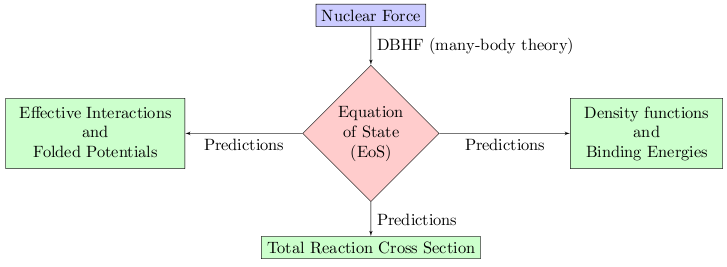
\includegraphics[width=17.6cm,height=6.5cm]{flowchart}
\caption{Schematic overview of poster. Using our nuclear force along with our many-body theory (DBHF) we calculate the equation of state (EoS) for isospin-asymmetric nuclear matter (IANM). In simple terms, IANM is a soup containing unequal amounts of protons and neutrons. Then, using our EoS we predict observables.\label{fig:flowchart}}
\end{center}
\end{figure}
\end{block}
\begin{block}{Motivation}
\begin{itemize}
\item Improving our understanding of nuclear matter, particularly in the presence of different neutron and proton concentrations, is one of the goals stated by the Nuclear Science Advisory Committee. This project generates predictions which can support present and future experimental effort with neutron-rich systems.  
\item \alert{Unfortunately, much of the nuclear landscape is still uncertain}. Today, our knowledge about nuclei is restricted to about 2500 of the potentially existing several thousand combinations of protons and neutrons.
\begin{figure}[H]
\begin{center}
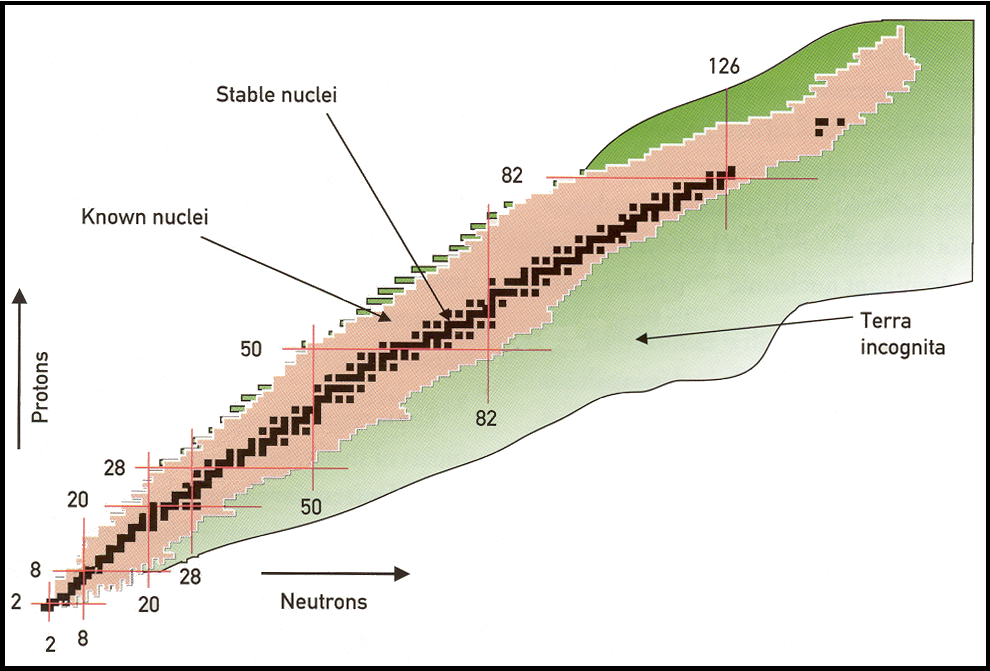
\includegraphics[width=9.5cm,height=6.5cm]{landscape}
\caption{The nuclear landscape, which is the playground for nuclear physics. Black squares indicate stable nuclei while the tan region represents roughly 2500 nuclei that have been synthesized. The green region is referred to as terra incognita because it's still unexplored.\label{fig:landscape}}
\end{center}
\end{figure}
\item \alert{The unknown region must be studied}. These unknown nuclei could be beneficial to nuclear medicine, or aid in our understanding of neutron stars and matter at the beginning of our universe.
\item A major experimental facility has been approved for construction (FRIB) in order to study these rare isotopes. \alert{Therefore, theoretical studies need to be underway}.
\item In addition, fundamental research like this has many spin-off technologies. For example, a driving factor in developing faster computers is that theoretical groups around the globe push the computational limit everyday. On a more local level, our group maintains a thirty core Beowulf cluster (or supercomputer) which is housed in the UI physics department. Thus, because of the theoretical nuclear physics group, the UI physics department now has a high end computing facility. 
\end{itemize}
\end{block}
\begin{block}{Methodology}
\begin{itemize}
\item \alert{We approach problems in an ab initio (from first principles) way as opposed to a phenomenological way}. That offers the opportunity to check
the predictive power of our theory.
\item In our ab initio approach, the fundamental nuclear force is used as input for our many-body calculations, without phenomenological contributions. 
\item We also strive to compare our theoretical calculations with experimental values.
\end{itemize}
\end{block}
\begin{block}{Main Components of the Model}
\begin{itemize}
\item \alert{Our starting point is a realistic nucleon-nucleon potential developed within a relativistic  scattering equation (Bonn potential)}. This potential describes the force between two interacting nucleons as taking place through the exchange of a boson. This scenario is depicted in Figure \ref{fig:feynman_diagram} as a Feynman diagram. In addition, see Figure \ref{fig:feynman_ball} for a simple analogy of the Feynman diagram.
\begin{figure}[H]
\begin{center}
\subfigure[]{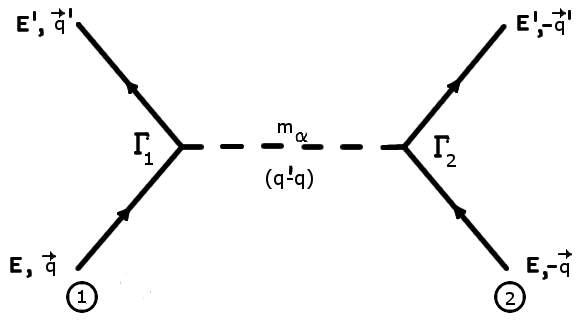
\includegraphics[width=5.5cm,height=5.5cm]{feynman}\label{fig:feynman_diagram}}
\hspace{5cm}
\subfigure[]{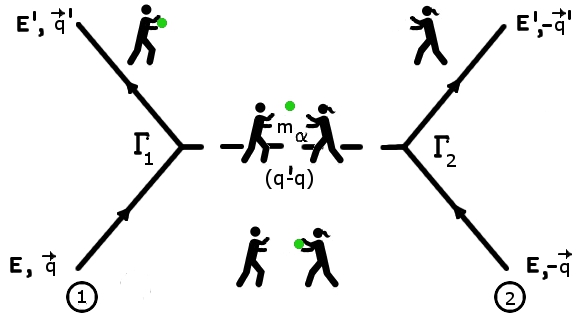
\includegraphics[width=5.5cm,height=5.5cm]{feynman_ball}\label{fig:feynman_ball}}
\caption{\subref{fig:feynman_diagram} Feynman diagram of a strong nucleon interaction mediated by the exchange of one boson. In the center of mass frame two nucleons have an initial momentum(energy) of $\pm q$($E$). After interacting via an exchange of a boson of mass $m_{\alpha}$ (which is the carrier of the strong force) the two nucleons emerge with a momentum(energy) of $\pm q^\prime$($E^\prime$). Time proceeds from bottom to top. \subref{fig:feynman_ball} Simple analogy of the Feynman diagram. (Bottom/middle) Two people (nucleons) are standing apart from each other and a ball (boson) is exchanged between them. (Top) Due to the exchange of the ball (boson) the two people (nucleons) are farther apart.\label{fig:feynman}}
\end{center}
\end{figure}
\item \alert{With a quantitative two-body interaction and the chosen many-body theory, namely} \alert{Dirac-Brueckner-Hartree-Fock (DBHF), we are ready to go into the many-body system}. Our playground is nuclear matter with different concentrations of protons and neutrons. This is commonly referred to as isospin-asymmetric nuclear matter (IANM). In simple terms, IANM is the stuff isospin-asymmetric nuclei are made of.
\end{itemize}
\end{block}
\end{column}
\begin{column}{0.32\paperwidth}
\begin{block}{Output of Model: EoS}
\begin{itemize}
\item \alert{The Equation of State (EoS) is a crucial player in the systems we consider}. It is the output of DBHF calculations. The EoS of IANM can be written in separable form as
\begin{equation}
e(\rho,\alpha) = e(\rho,\alpha = 0) + e_{sym}(\rho)\alpha^2,
\end{equation}
where $\rho=\rho_n + \rho_p$ is the total density, $\alpha = \frac{\rho_n - \rho_p}{\rho}$ is the neutron excess, and $e_{sym}=e(\rho,\alpha=1)-e(\rho,\alpha=0)$ is known as the symmetry energy. $\rho_{n(p)}$ are the neutron(proton) density functions.
\begin{figure}[H]
\begin{center}
\subfigure[]{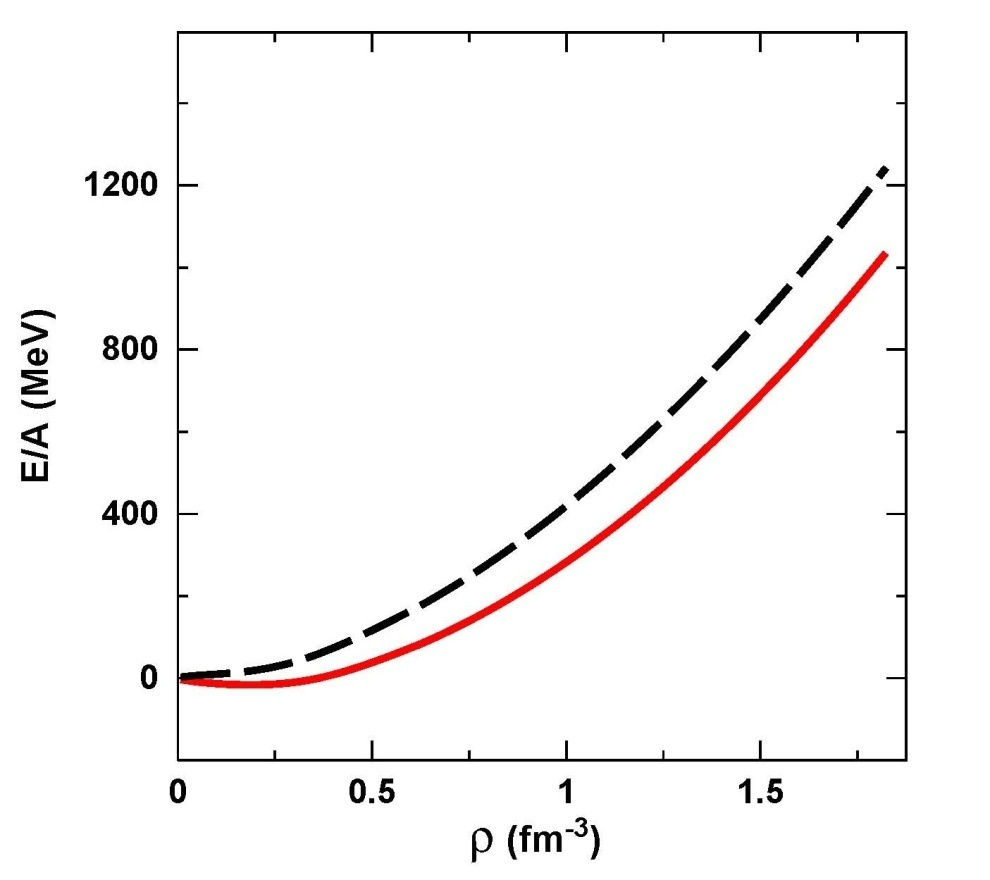
\includegraphics[width=12cm,height=10cm]{eos}\label{fig:eos}}
\hspace{5cm}
\subfigure[]{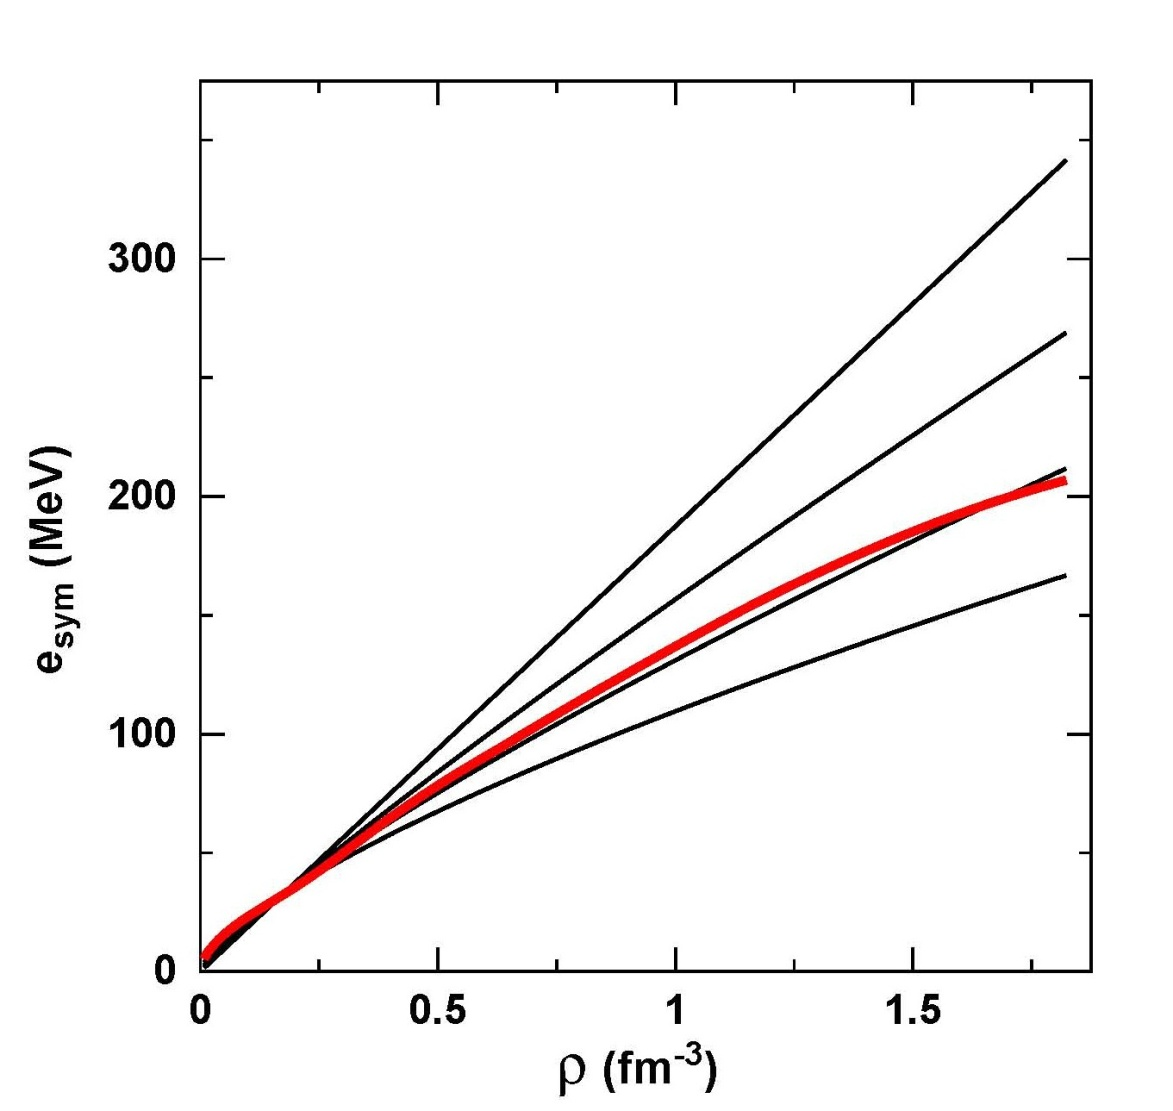
\includegraphics[width=12cm,height=10cm]{esym}\label{fig:e_sym}}
\caption{\subref{fig:eos} Plot of the EoS $e(\rho,\alpha)$ as a function of density. The black (dashed) curve is for $\alpha = 1$ while the red (solid) curve is for $\alpha = 0$. \subref{fig:e_sym} Plot of $e_{sym}$ as a function of density. The red curve is the EoS as derived through DBHF predictions. The black curves are commonly used parameterizations.\label{eos_e_sym}}
\end{center}
\end{figure}
\item \alert{The uncertainty in our knowledge of the EoS is apparent through the $e_{sym}$ term}. Our predictions of the EoS (for both symmetric and asymmetric matter), are well within available constraints. However, more and better constraints are needed, especially at high density, where model dependence is largest. There are open questions, for both theorists and experimentalists.
\end{itemize}
\end{block}
\begin{block}{EoS Predictions: nuclear densities}
\begin{itemize}
\item \alert{From the EoS of IANM one can determine the neutron and proton density functions}.
\begin{figure}[H]
\begin{center}
\subfigure[]{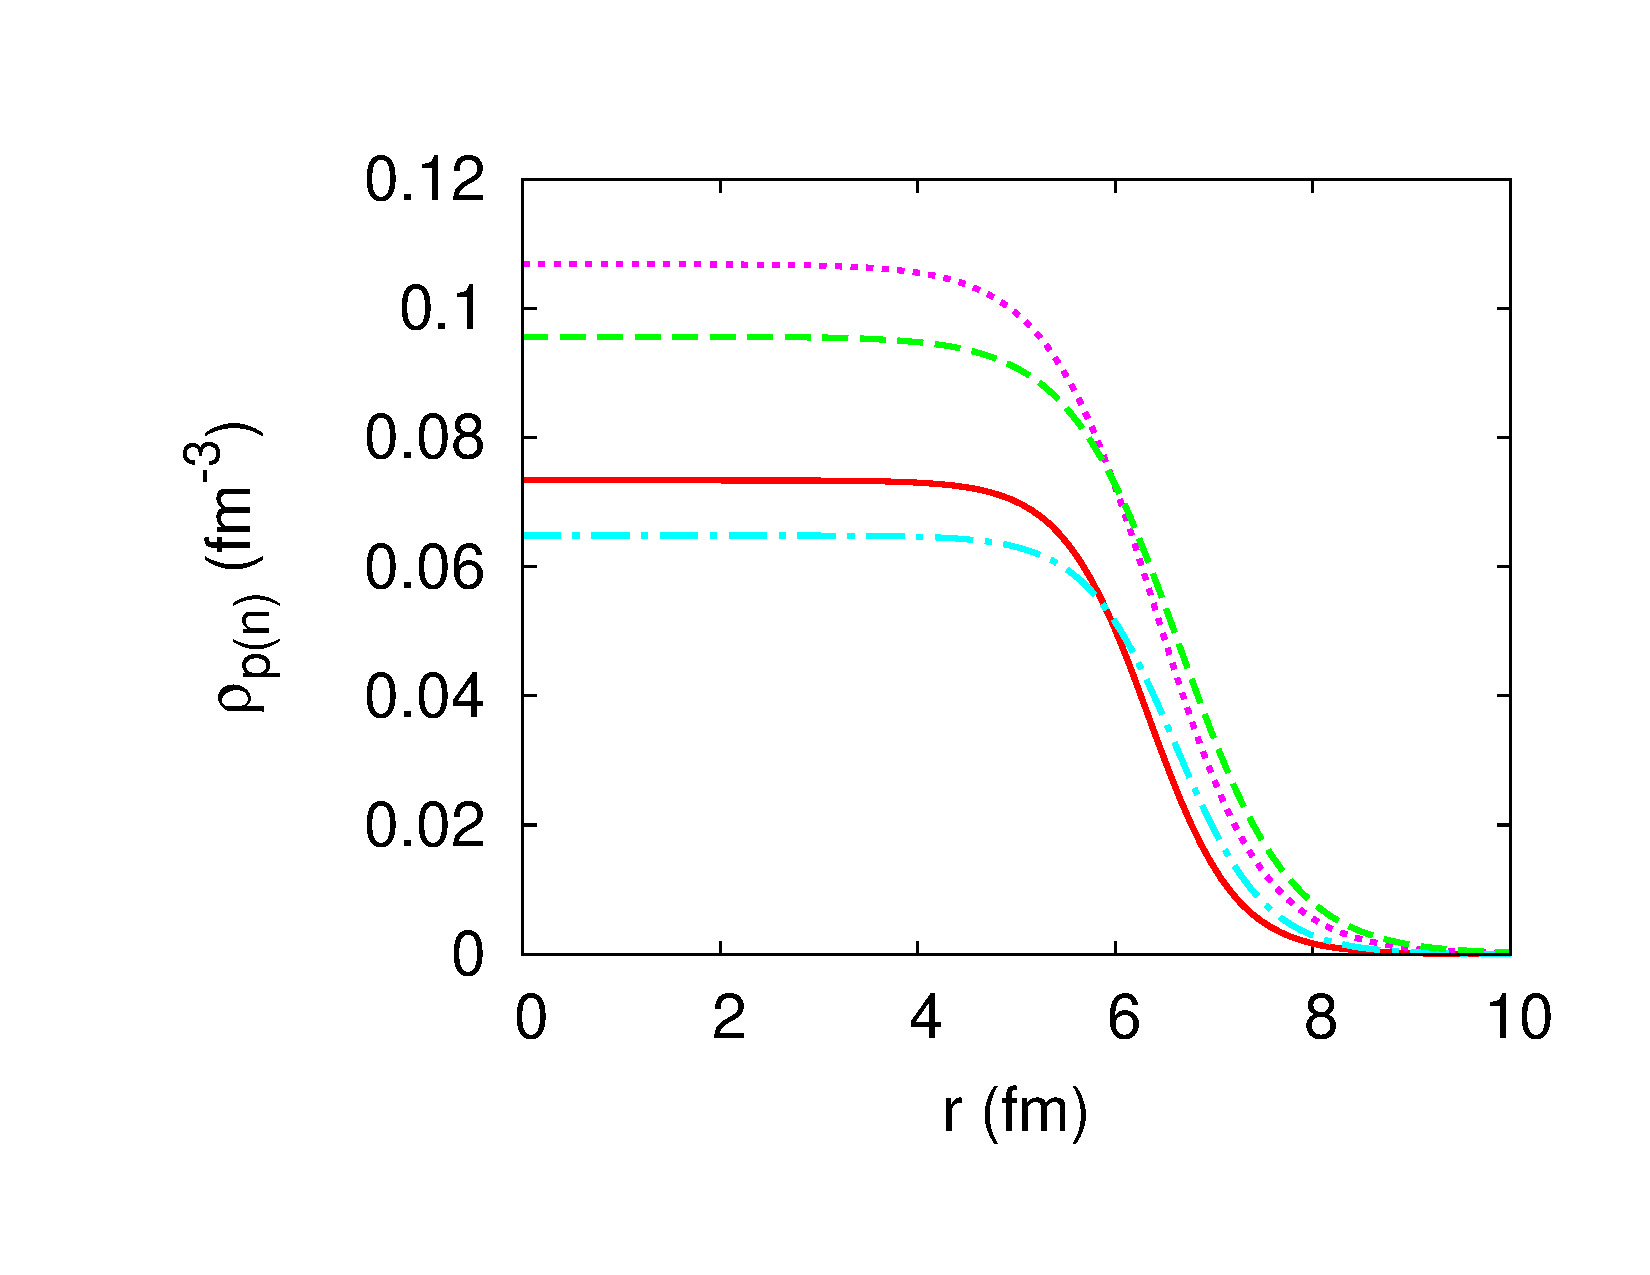
\includegraphics[width=12.7cm,height=10.7cm]{208Pb_rho_Bonn}\label{fig:rho_theo}}
\hspace{5cm}
\subfigure[]{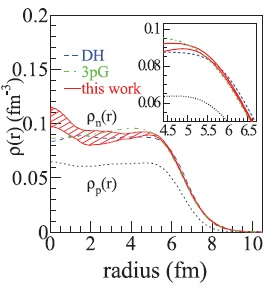
\includegraphics[width=9.7cm,height=9.7cm]{rho_exp}\label{fig:rho_exp}}
\caption{\subref{fig:rho_theo} $^{208}$Pb density functions used to describe the proton (Bonn A: solid red curve and Bonn B: dash dotted blue curve) and neutron (Bonn A: dotted pink curve and Bonn B: dashed green curve) densities. \subref{fig:rho_exp} Experimentally measured $^{208}$Pb neutron and proton density functions. Experimental results from \textit{J. Zenihiro et al., Phys. Rev. C 82 044611, (2010)}.\label{density}}
\end{center}
\end{figure}
\item Density functions as well as binding energies $B$ are calculated via a liquid drop model,
\begin{equation}
-B = \int_{\mathbb{R}^3} e( \rho(\bvec{r}), \alpha(\bvec{r}) ) \rho(\bvec{r}) + f_0 \abs{ \nabla \rho(\bvec{r}) }^2 \dd^3 r + \frac{e^2}{8 \pi \epsilon_o}\int_{\mathbb{R}^6} \frac{ \rho_p(\bvec{r}) \rho_p(\bvec{r}^\prime)}{\abs{\bvec{r}-\bvec{r}^\prime}} \dd^3 r \dd^3 r^\prime.
\label{eq:binding}
\end{equation}
A typical value for $f_0$ is $70$ $\mathrm{MeV} \, \mathrm{fm}^{-5}$. \alert{Also, our EoS appears under the integrand of the first term}.
\item The neutron and proton density functions are usually assumed to have the functional form
\begin{equation}
\rho_i(r) = \frac{N_i}{1+\exp\rb{\frac{r - a_i}{c_i}}} \quad \text{for $i=n,p$}.
\end{equation}
Since $N_i$ is a normalization constant there are two parameters in this function $a_i$ and $c_i$. Parameter values are chosen in order to maximize the binding energy. Therefore, the problem of finding binding energies and density functions is reduced to global optimization.
\item From the neutron/proton density functions we can calculate and compare RMS radii
\begin{equation}
 \avg{r^2_{pt}}_i^{\sfrac{1}{2}} = \sqrt{\frac{4 \pi}{N_i} \int_0^\infty r^4 \rho_i(r) \dd r} \quad \text{for $i=n,p$},
\end{equation}
and neutron skins
\begin{equation}
S_n=\avg{r^2_{pt}}_n^{\sfrac{1}{2}}-\avg{r^2_{pt}}_p^{\sfrac{1}{2}}.
\end{equation}
\begin{table}[H]
\caption{Theoretical and experimental: proton/neutron RMS radii, neutron skins and binding energies for $^{208}$Pb. All values in fm unless stated otherwise.}
\label{table:theo_exp}
\large
\begin{center}
\begin{tabular}{llllll}
\hline\hline
& $\langle r^2_{pt} \rangle_n^{1/2}$ & $\langle r^2_{pt} \rangle_p^{1/2}$ & $S_n$ & $B$ (MeV) &\\ \hline
\multirow{1}{*}{Theo. Bonn A} & 5.36 & 5.17 & 0.19 & 8.36 &\\
\multirow{1}{*}{Theo. Bonn B} & 5.56 & 5.39 & 0.17 & 7.19 &\\
\multirow{1}{*}{Exp.} & $^\text{a}5.653^{+0.054}_{-0.063}$ & $^\text{a}5.442(2)$ & $^\text{a}0.211^{+0.054}_{-0.063}$ & $^\text{b}$7.87 &\\
\hline\hline
\multicolumn{5}{l}{$^\text{a}$\small{\textit{J. Zenihiro et al., Phys. Rev. C 82 044611, (2010).}}} \\
\multicolumn{5}{l}{$^\text{b}$\small{\textit{U.S. National Nuclear Data Center, BNL, ``Nudat 2.3'', online (2007).}}}
\end{tabular}
\end{center}
\end{table}
\end{itemize}
\end{block}
\end{column}
\begin{column}{0.32\paperwidth}
\begin{block}{EoS Predictions: total reaction cross section}
\begin{itemize}
\item \alert{Using density functions we can calculate the total reaction cross section $\sigma_R$}.
\item The total reaction cross section is of fundamental importance; for example, they are used in the design of nuclear reactors. $\sigma_R$ is calculated via
\begin{subequations}
\label{eq:sigma_R}
\begin{align}
\sigma_R & = 2 \pi \int_0^\infty (1 - T(b)) b \dd b, \\
T(b) & = \exp \sqb{-\int_{\mathbb{R}^4} f(\abs{\bvec{r}_T - \bvec{r}_P}) \sum_{i,j = n,p} \sigma_{ij} \rho^{(T)}_{z,i}(\abs{\bvec{r}_T}) \rho^{(P)}_{z,j}(\abs{\bvec{r}_P-\bvec{b}}) \dd^2 r_T \dd^2 r_P}.
\end{align}
\end{subequations}
\end{itemize}
The function $f(\abs{\bvec{r}_T - \bvec{r}_P})$ is usually taken to be of Gaussian form. Additionally, $\sigma_{ii}$($\sigma_{ij}$) are the nucleon-nucleon cross sections for scattering of identical(non-identical) nucleons. Finally, $\rho^{(T)}_{z,i}$ and $\rho^{(P)}_{z,j}$ are calculated using our density functions which were obtained from Eq. \ref{eq:binding}. More explicitly they are defined as
\begin{subequations}
\begin{align}
\rho^{(T)}_{z,i}(\abs{\bvec{r}_T}) & = \int_{\mathbb{R}} \rho^{(T)}_i \rb{ \sqrt{  \bvec{r}_T^2 + z^2  } } \dd z, \\
\rho^{(P)}_{z,j}(\abs{\bvec{r}_P - \bvec{b}}) & = \int_{\mathbb{R}} \rho^{(P)}_j \rb{ \sqrt{  \abs{ \bvec{r}_P - \bvec{b} } + z^2  } } \dd z.
\end{align}
\label{eq:rho_ij}
\end{subequations}
\begin{figure}[H]
\begin{center}
\subfigure[Calcium isotopes]{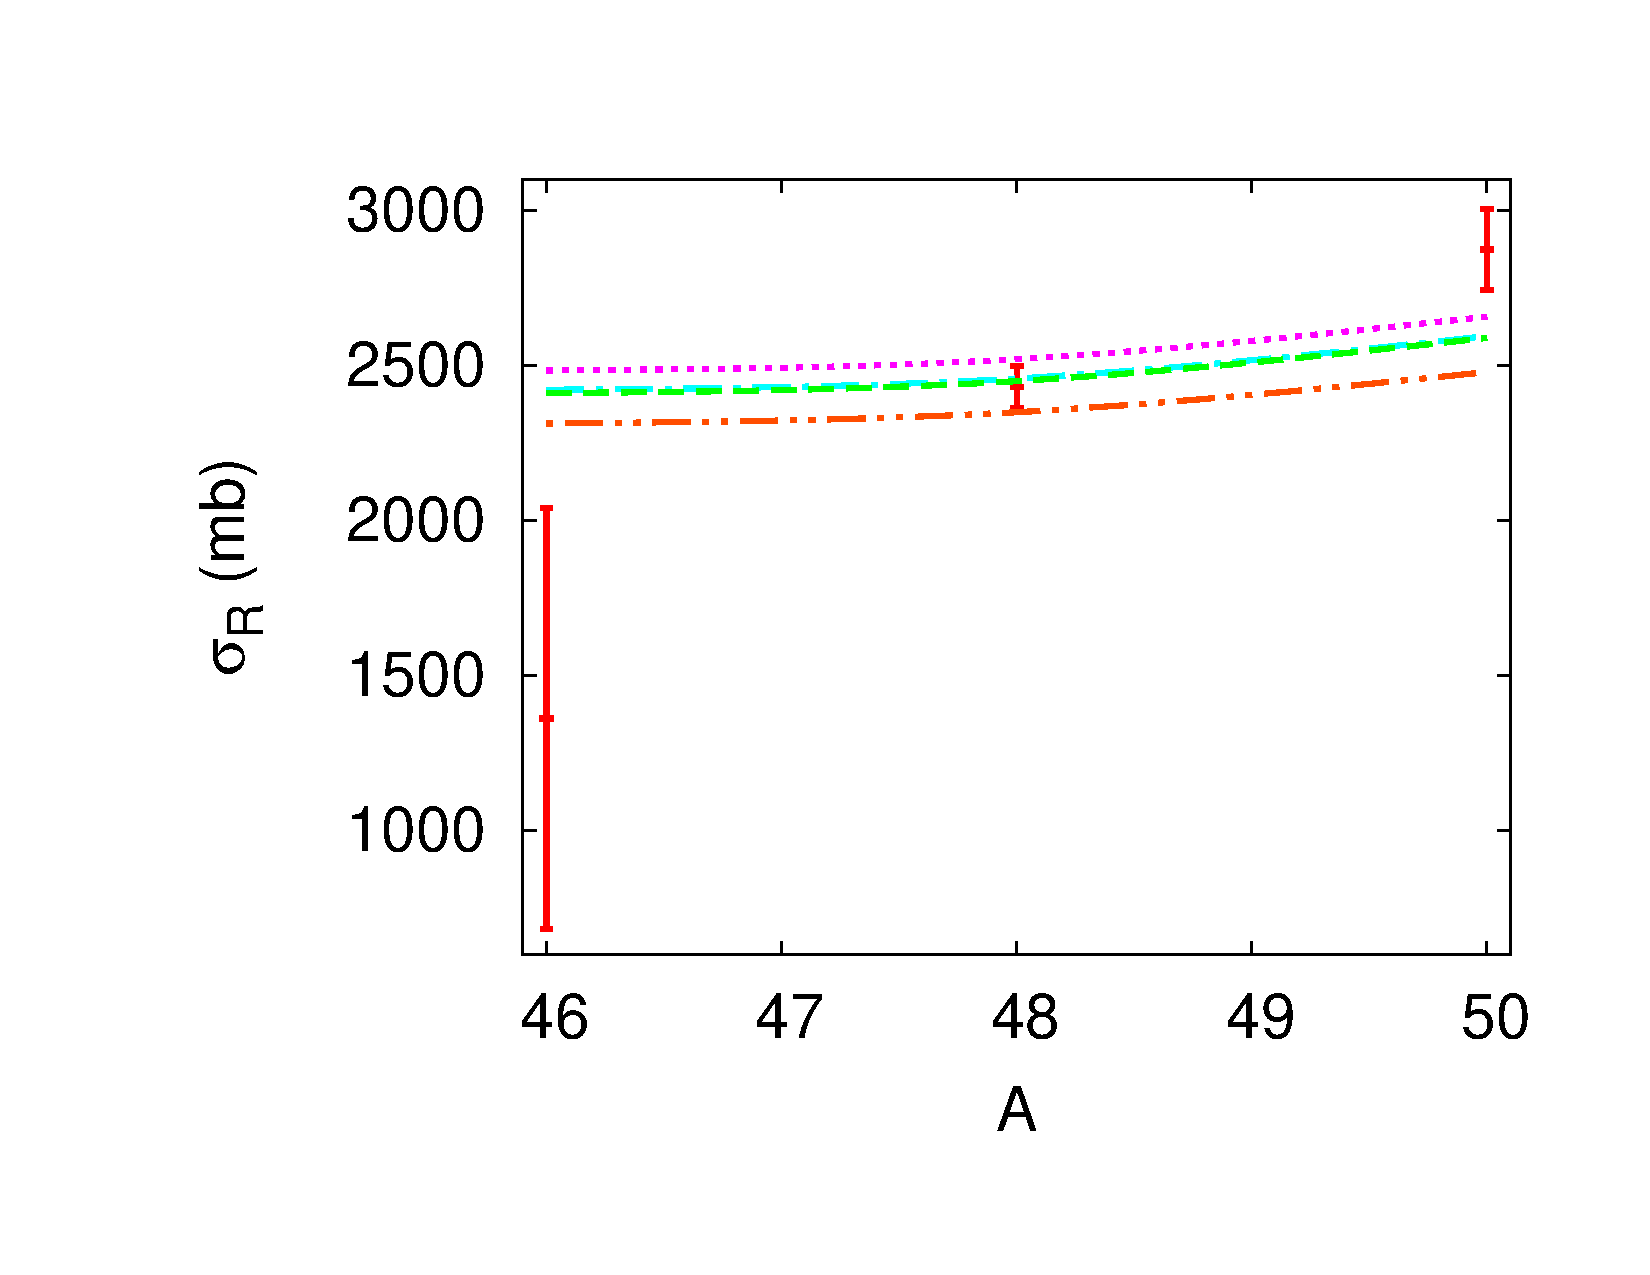
\includegraphics[width=11cm,height=9cm]{Ca}\label{fig:ca}}
\hspace{5cm}
\subfigure[Argon isotopes]{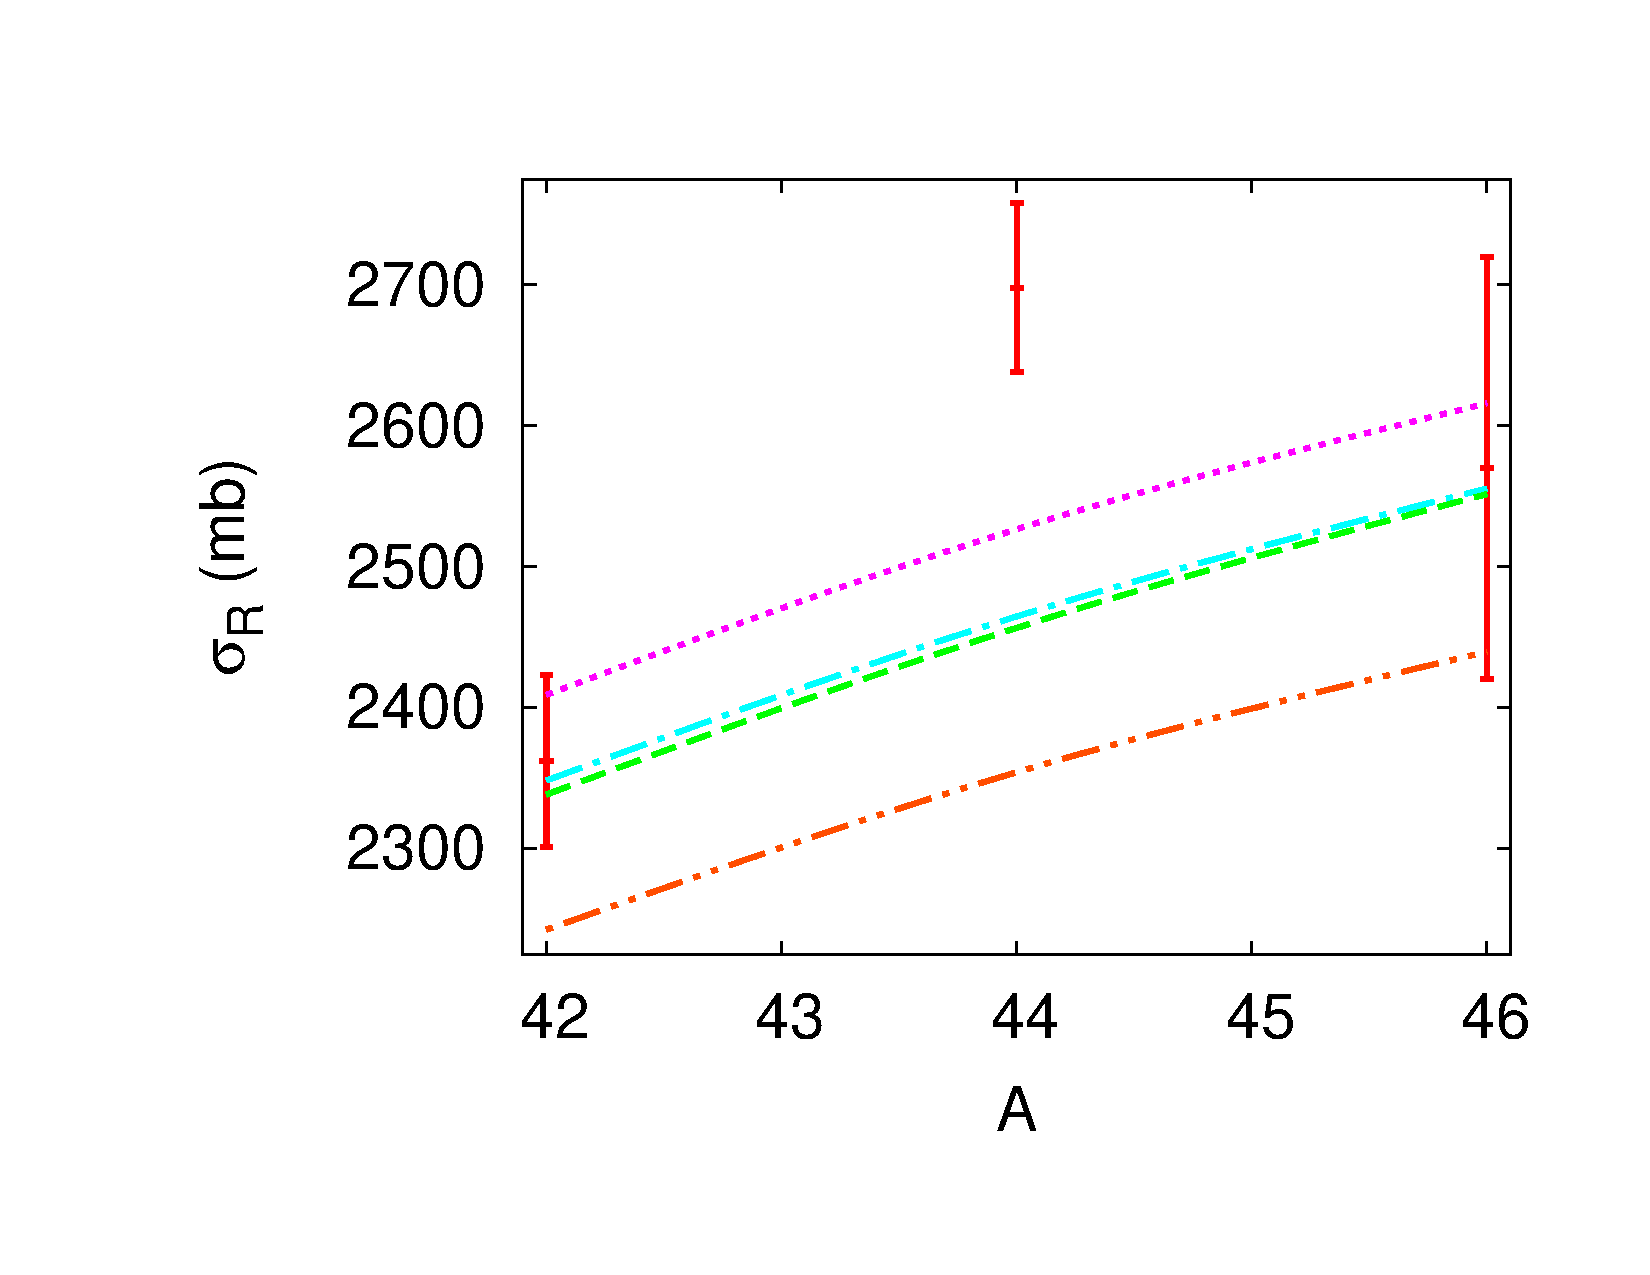
\includegraphics[width=11cm,height=9cm]{Ar}\label{fig:ar}}
\caption{Plot of the reaction cross section $\sigma_R$ as a function of the mass number. The different curves represent different models we used to calculate $\sigma_R$. Data from: \textit{I. Locot et al., Phys. Rev. C 56, 250 (1997)}.\label{ca_ar}}
\end{center}
\end{figure}
\end{block}
\begin{block}{EoS Predictions: current work on effective interactions}
\begin{itemize}
\item \alert{Our current work has a solid foundation in what we have discussed so far}.
\item In our microscopic approach the effective interaction (a nucleon-nucleon interaction modified by the presence of the nuclear medium) is the solution of the Bethe-Goldstone integral equation,
\begin{equation}
\braket{\lambda_1^\prime \lambda_2^\prime|G(\bvec{q},\bvec{q}^\prime)|\lambda_1 \lambda_2}  = \braket{\lambda_1^\prime \lambda_2^\prime|V(\bvec{q},\bvec{q}^\prime)|\lambda_1 \lambda_2} + \sum_{h_1,h_2=\pm \frac{1}{2}}\frac{1}{2}\int_{\mathbb{R}^3} \frac{\braket{\lambda_1^\prime \lambda_2^\prime|V(\bvec{k},\bvec{q}^\prime)|h_1 h_2}\braket{h_1 h_2 |G(\bvec{q},\bvec{k})|\lambda_1 \lambda_2} Q(\bvec{k},\bvec{P}) }{E_q - E_k + i \epsilon} \dd^3 k
\quad \text{for $\lambda_1^\prime,\lambda_2^\prime,\lambda_1,\lambda_2 = \pm \frac{1}{2}$}.
\label{eq:G}
\end{equation}
\end{itemize}
The operator $Q(\bvec{k},\bvec{P})$ is referred to as the Pauli operator ($\bvec{P}$ is one half the center of mass momentum) and prevents scattering into occupied states. For free space it's set to unity. The vectors $\bvec{q}$, $\bvec{k}$, $\bvec{q}^\prime$ are the initial, intermediate, and final three momentum respectively. The terms $E_q$ and $E_k$ are relativistic energies obtained from
\begin{equation}
E_p = \sqrt{p^2 + ({m^\ast})^2},
\end{equation}
where one has to be careful to use the in medium mass $m^\ast$ for the scattered nucleon.
\begin{itemize}
\item Currently we have the nuclear potential $\braket{\lambda_1^\prime \lambda_2^\prime|V(\bvec{q},\bvec{q}^\prime)|\lambda_1 \lambda_2}$ programed and modified to fully discriminate between protons and neutrons. Now we are working on solving for the matrix elements $\braket{\lambda_1^\prime \lambda_2^\prime|G(\bvec{q},\bvec{q}^\prime)|\lambda_1 \lambda_2}$.
\item Eq. \ref{eq:G} is non-trivial to solve. It's a coupled set of six linear Fredholm integral equations of the second kind. By converting the system of integral equations to a vector matrix equation i.e. $\bvec{A}\bvec{x}=\bvec{b}$, the solution for $\braket{\lambda_1^\prime \lambda_2^\prime|G(\bvec{q},\bvec{q}^\prime)|\lambda_1 \lambda_2} $ is obtained by matrix inversion.
\item The Bethe-Goldstone equation has been solved many times using an established procedure in quantum mechanics; the so-called partial wave expansion. This method allows one to eliminate the angular variables from the kernel of the equation and thus reduce the number of integrations.
\item \alert{We wish to solve this set of integral equations in 3D space}. While the numerics may be more involved, it will allow us to remove a typical approximation on the Pauli operator.
\item Once this improved effective interaction is available, it can be used for many things, nuclear reactions being the most obvious one. For instance, in microscopic calculations of nucleon-nucleus scattering, the effective interaction is directly used to construct the so-called ``folded potential'', where the interaction is folded with the nuclear density to provide the average potential felt by the projectile nucleon.
\item \alert{Our current work is consistent with everything we have discussed so far} since nuclear densities, of which our group calculates through our EoS are needed to calculate the ``correct'' folded potentials $U_n(p)$
\begin{subequations}
\begin{align}
U_n & = G_{nn} \rho_n + G_{np} \rho_p, \\
U_p & = G_{p} \rho_p + G_{pn} \rho_n.
\end{align}
\label{eq:folded}
\end{subequations}
\item Implications of our modified or ``correct'' folded potentials come from the fact that proton densities can be measured while neutron densities can at most be extracted indirectly. For moderately neutron-rich nuclei people have assumed that neutron densities have the same shape as protons densities. But our modified folded potentials with the inclusions of IANM may be important in a highly neutron-rich environment. We will explore to which extent this is the case.
\end{itemize}
\end{block}
\begin{block}{Conclusion}
Much of the nuclear landscape is still unknown. The FRIB experimental program is expected to improve dramatically our knowledge of the nuclear chart and its boundaries. At the same time, newly discovered rare isotopes will be helpful in medical diagnostics and treatment. Parallel theoretical efforts are important and timely! Our microscopic studies of neutron-rich nuclear matter are closely related to the physics of unstable nuclei through the equation of state, which enters into predictions of nuclear densities, reaction cross sections, and effective interactions. We stress again the importance of ab initio calculations towards a better understanding of the nuclear force in the many-body system.
\end{block}
\begin{block}{acknowledgments}
The authors would like to thank the U.S. Department of Energy for support.
\end{block}
\end{column}
\end{columns}
\end{frame}
\end{document}
